\documentclass[ieeebib]{class/IGPthesis} % Use the option kbib if you prefer AAAI style citations
\usepackage[utf8]{inputenc}
\usepackage[english]{babel}
\usepackage{amsmath}
\usepackage{amsfonts}
\usepackage{amssymb}
\usepackage{amsthm}
\usepackage{graphicx}
\usepackage{subcaption} % For complex figures
\usepackage[titletoc, header, page]{appendix}
\usepackage{graphicx}
\usepackage{array}      % For fancy tables
\usepackage{booktabs}   % For formal tables
\usepackage{longtable}  % For long tables
\usepackage{lipsum}
\usepackage{siunitx}    % International System of Units

% MY'25: Removing breakurl because it was causing problems
% MY'25: DO NOT include natbib or any other bibliography package here, it will be handled by the IGPthesis class
\usepackage{datetime}   % To manage date format
\usepackage[pdfusetitle]{hyperref}
\usepackage{setspace}   % To configure dobule/single space
\usepackage{multirow}
\usepackage{pdflscape} 
\usepackage{afterpage}
\usepackage{capt-of}% or use the larger `caption` package
\usepackage{pdfpages} %include pdf files in appendix
\usepackage{stackengine} %for overlapping figures
\usepackage{epigraph} % for highlights

% MY'25: Here's some additional package I found useful:
\usepackage[nohyperlinks]{acronym}             % Easily manage acronyms
\usepackage{adjustbox}                         % Rotate figures by 90 degrees
\usepackage{algorithmic}                       % Provide algorithm environment
\usepackage[linesnumbered,ruled]{algorithm2e}  % Nicer algorithms

% For block quote colored:
\usepackage[most]{tcolorbox}
\definecolor{block-gray}{gray}{0.85}
\newtcolorbox{blockquote}{colback=block-gray,grow to right by=-1mm,grow to left by=-1mm,boxrule=0pt,boxsep=0pt,breakable}

%%% Handle hypenation for long words
\tolerance=1
\emergencystretch=\maxdimen
\hyphenpenalty=10000
\hbadness=10000

% MY'24: the following can be helpful when debugging margins
%\geometry{showframe}

% Title goes here
\title{Thesis Title}

% Name should be in block (uppercase) letters as it appears on your matriculation card
\author{SURNAME GIVEN-NAMES}

% Affiliation format:
% Line 1 - "Interdisciplinary Graduate Programme"
% Line 2 - Research Center Name
\affiliation{Interdisciplinary Graduate Programme \\ Energy Research Institute @ NTU}
\affilogo{class/logos/logo_ntu.png}

\TypeOfDocument{A thesis submitted to the Nanyang Technological University in partial fulfilment of the requirement for the degree of Doctor of Philosophy}

%% Date without the day of the month
\newdateformat{titledate}{\THEYEAR}
\newdateformat{signaturedate}{\THEDAY\hspace{0.5em}\shortmonthname[\THEMONTH] \THEYEAR}
\date{\titledate\today}

% MY'25: Adding Theorem and Lemma environemnts
\newtheorem{theorem}{Theorem}
\newtheorem{lemma}{Lemma}

\begin{document}
    %% This command generates all the pages before Chapter 1
    %% Cover, Abstract, Declaration, Acknowledgements, Contents
    \makefrontmatter

    %% Contents are still in roman numbers, don't touch this
    \cleardoublepage

    %% Arabic numbers from Chapter 1 to the end.
    \pagenumbering{arabic}

    \ifdefined\isdraft
        \doublespacing
    \else
        \onehalfspacing
    \fi

    %% Chapters. Include here all your chapters
    \chapter[Introduction]{Introduction}\label{chap-intro}

%%%%%%%%%%%%%%%%%%%%%%%%%%%%%%%%%%%%%%
\section{Background}
%%%%%%%%%%%%%%%%%%%%%%%%%%%%%%%%%%%%%%

It is a good idea to discuss the structure of the report with your supervisor rather early in your writing.

%%%%%%%%%%%%%%%%%%%%%%%%%%%%%%%%%%%%%%
\section{Sample Table}

As a recommendation, use regular paragraph text in the tables, bold headings and avoid vertical lines (see Table \ref{tab:margins}). 

\begin{table}
\centering
\caption{Text margins for A4.}\label{tab:margins}
\begin{tabular}{cc}
\hline
\textbf{margin} & \textbf{space} \\
\hline 
top &  3.0cm\\ 
bottom & 3.0cm \\ 
left (inside) & 2.5cm \\ 
right (outside) & 2.5cm \\ 
binding offset & 1.0cm \\ 
\hline 
\end{tabular} 
\end{table}

%%%%%%%%%%%%%%%%%%%%%%%%%%%%%%%%%%%%%%
\section{Sample Figure}

As a recommendation, use vector graphics in figures (Figure \ref{fig:vectorg}), rather than bitmaps (Figure \ref{fig:rasterg}). Text within figures usually looks better with sans-serif fonts.  I prefer to use \texttt{width} to adjust the width of figures and set sizes relative to the line width instead of using \texttt{scale}.

\begin{figure}
\centering
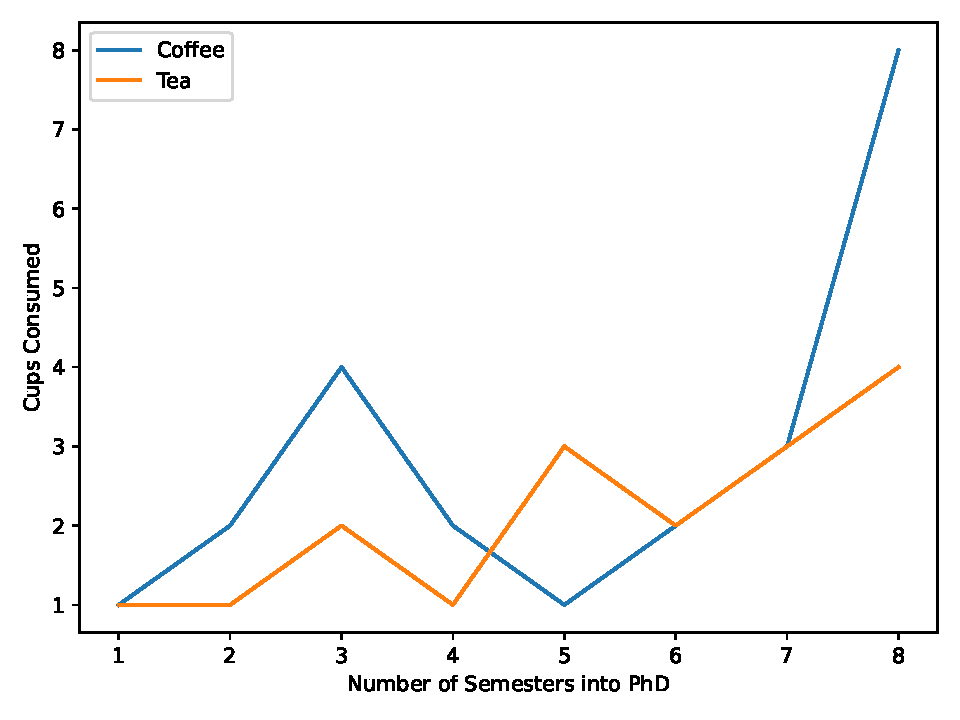
\includegraphics[width=1\linewidth]{Figures/Figure_1.pdf} 
\caption{A PDF vector graphics figure. Notice the numbering and placement of the caption. The caption text is indented 2.0cm from both left and right text margin.}\label{fig:vectorg}
\end{figure}

\begin{figure}
\centering
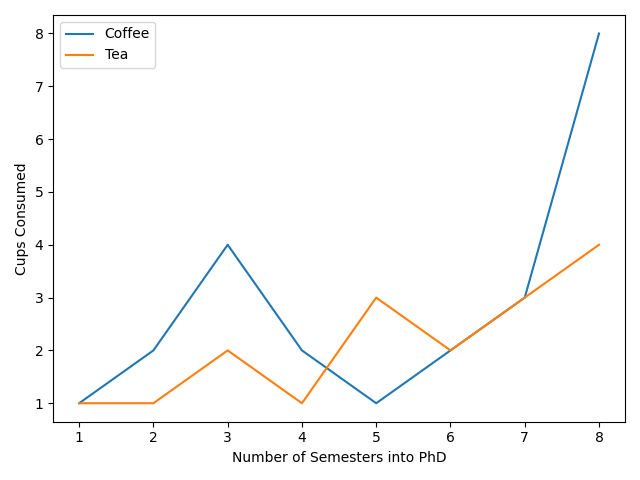
\includegraphics[width=1\linewidth]{Figures/Figure_1.png} 
\caption{A PNG bitmap figure. Notice the bad quality of such an image when scaling it. Sometimes bitmap images are unavoidable, such as for screen dumps.}\label{fig:rasterg}
\end{figure}

\begin{figure}
\centering
\begin{adjustbox}{
  addcode={\begin{minipage}{\width}}{
    \caption{You can use the adjustbox environment to rotate an image if you have trouble fitting it on a page.}\label{fig:rotated}
    \end{minipage}
  },rotate=90,center}
  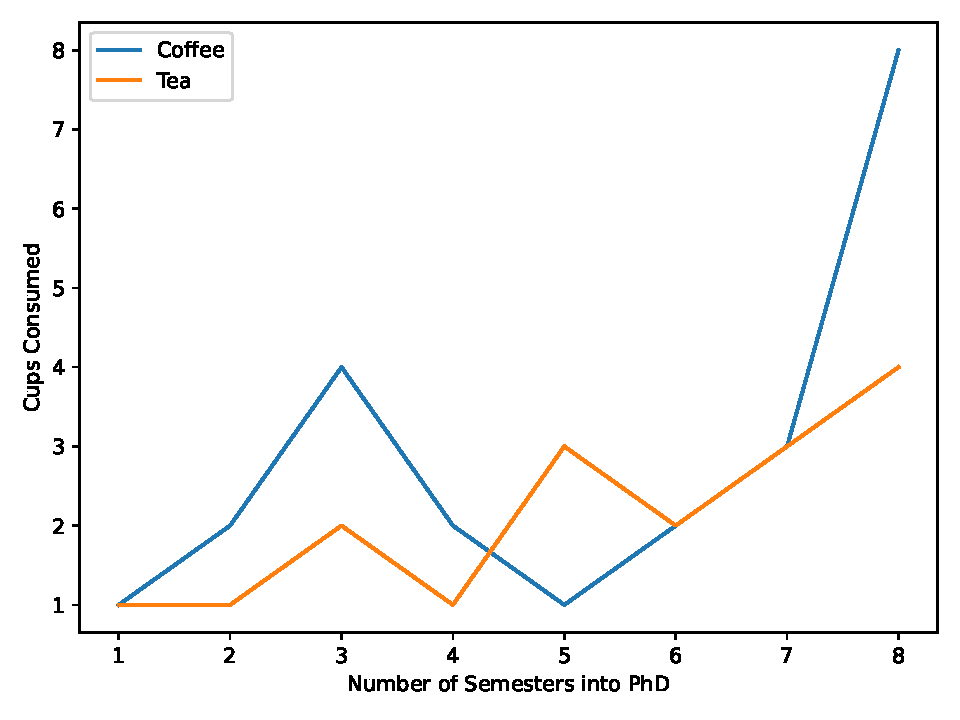
\includegraphics[width=1\linewidth]{Figures/Figure_1.pdf}
\end{adjustbox}
\end{figure}

\begin{figure}
\centering
\begin{subfigure}{0.45\textwidth}
  \centering
  \captionsetup{width=0.9\linewidth}
  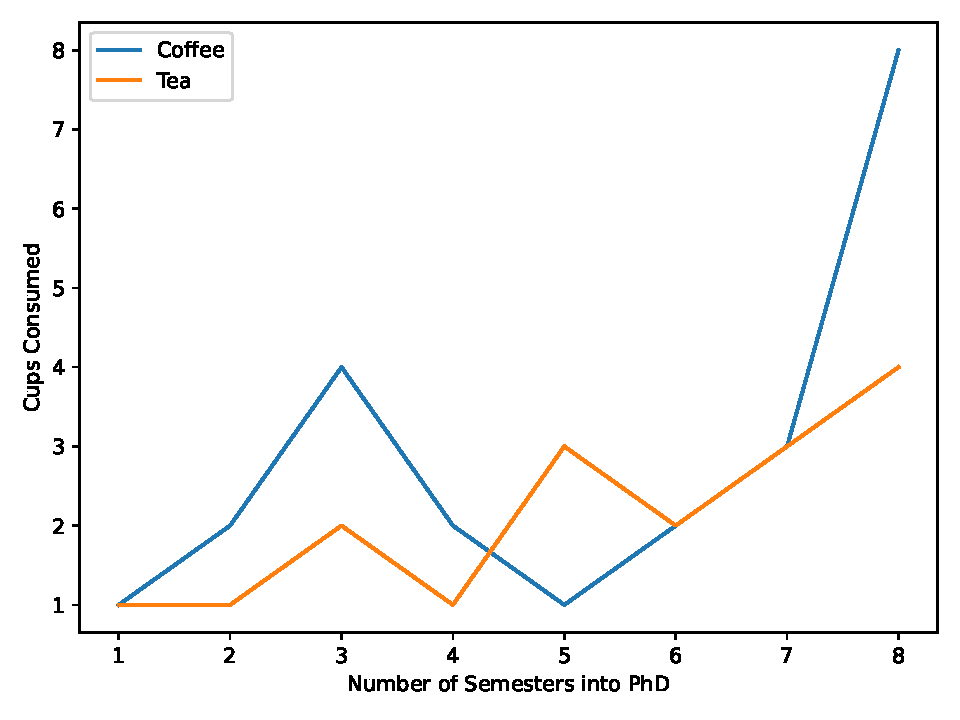
\includegraphics[width=1\linewidth]{Figures/Figure_1.pdf}
  \caption{This is a sub-caption.}
  \label{subfig:a}
\end{subfigure}
\begin{subfigure}{0.45\textwidth}
  \centering
  \captionsetup{width=0.9\linewidth}
  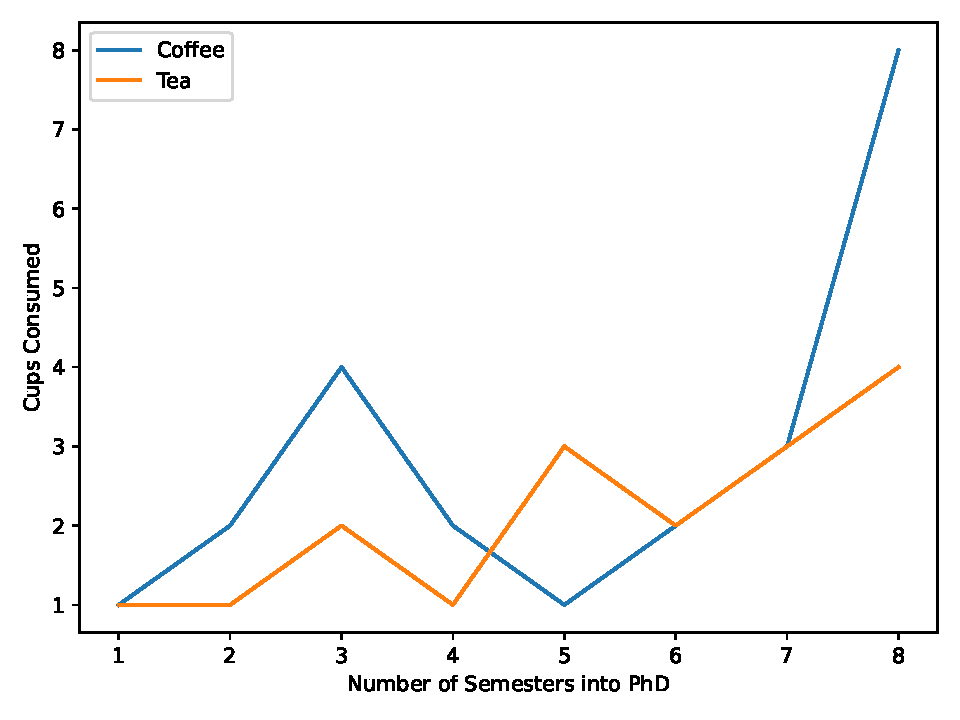
\includegraphics[width=1\linewidth]{Figures/Figure_1.pdf}
  \caption{This is another sub-caption.}
  \label{subfig:b}
\end{subfigure}
\caption{Caption for the entire figure.  I find the sub-figure captions look better if the width is set to 0.9.}
\label{fig:subfigs}
\end{figure}

%%%%%%%%%%%%%%%%%%%%%%%%%%%%%%%%%%%%%%
\section{Sample Equation}

You are free to use in-text equations and formulae, usually in \textit{italic serif} font. For instance: $S = \sum_i a_i$. We recommend using numbered equations (e.g. Equation \ref{eqn:emc1} when you do need to refer to the specific equations:

\begin{equation}
E = \int_0^{\delta} P(t) dt \quad \longleftrightarrow \quad E = m c^2
\label{eqn:emc1}
\end{equation} 

%%%%%%%%%%%%%%%%%%%%%%%%%%%%%%%%%%%%%%
\section{Sample Algorithm}

I like to use the Algorithm2e package for pseudocode like in the ACM journal template (e.g. Algorithm~\ref{alg:binary_search}).

\begin{algorithm}
\caption{Find the index of an element in an ordered list.}
\label{alg:binary_search}
\KwIn{Ordered list $L = \{ L_0 \dots L_n \}$, and a value $v$}
\KwOut{Index $m$ of value $v$ in $L$}
$l = 0$;
$r = n - 1$;
\While{$L_m \neq v$}{
  $m = \lfloor (l + r) / 2 \rfloor$;
  \uIf{$L_m < v$}{
    $l = m + 1$;
  }
  \uElseIf{$L_m > v$}{
    $r = m - 1$;
  }
  \uElse{
    \Return $m$;
  }
}
\Return $\emptyset$;
\end{algorithm}

%%%%%%%%%%%%%%%%%%%%%%%%%%%%%%%%%%%%%%
\section{Theorems, Lemmas, and Proofs}

\begin{theorem}
    Theorems are defined like this.
\end{theorem}
\begin{proof}
    The proof environment should immediately follow.
\end{proof}

\begin{lemma}
    Lemmas can be defined in a similar manner.
\end{lemma}
\begin{proof}
    This is the proof associated with the lemma.
\end{proof}

    \chapter[Project 1 Sample]{Project 1 Sample}\label{chap-sample}

%%%%%%%%%%%%%%%%%
\section{Abstract}

This is a sample structure based on personal recommendations, and not on NTU guidelines.

%----------------
\section{Introduction}\label{section-intro}
%----------------
State the objectives of the work and provide an adequate background, avoiding a detailed literature survey or a summary of the results. You can cite single authors \cite{connor2006inversion} or multiple authors (e.g. \cite{volentik2010modeling, costa2012, bonadonna2013}.  Note that the \texttt{citep} and \texttt{citet} citation styles are not available if the IEEE bibliography format is selected.

%----------------
\section{Methods}\label{section-methods}
%----------------

Provide sufficient detail to allow the work to be reproduced. Methods already published should be indicated by a reference: only relevant modifications should be described. 

%----------------
\section{Results and Discussion}\label{section-results} 
%----------------
Results should be clear and concise. 

\subsection{Test case}

%----------------
\section{Conclusions}\label{section-conclusion}
%----------------

The main conclusions of the study may be presented in a short Conclusions section, which may stand alone or form a subsection of a Discussion or Results and Discussion section.


    \chapter[Project 2 Sample]{Project 2 Sample}\label{chap-sample-2}

%%%%%%%%%%%%%%%%%
\section{Sample section}

%%%%%%%%%%%%%%%%%
\subsection{Sample subsection}

%%%%%%%%%%%%%%%%%
\subsubsection{Sample subsubsection}
    \chapter[Conclusions]{Conclusions}\label{chap-conc}

Your conclusions go here. You can link to specific chapters, for instance, Chapter \ref{chap-intro}, \ref{chap-sample}, and \ref{chap-sample-2}.


\begin{center} \begin{blockquote}
I also like to highlight specific messages using block quotes like this.
\end{blockquote} \end{center}


    %% Bibliography using bibtex
    \makebibliography{refs.bib}

    %% Appendices. If you don't have any appendices, comment the appendices section
    \begin{appendices}

        %% Include here all your appendices
        \chapter{Title of your first appendix}

\section{Subsection title} \label{app-a}

This is your first Appendix section.

% If you want to add a pdf file in the appendix, use the following command
%\includepdf[pages={1}]{papers/popsci.pdf}
        \chapter{Title of your second appendix}

\section{Subsection title 1} \label{app-b-1}

You can insert your Appendix B here.

\section{Subsection title 2} \label{app-b-2}

You can add more sections in your Appendix.

    \end{appendices}

\end{document}


